
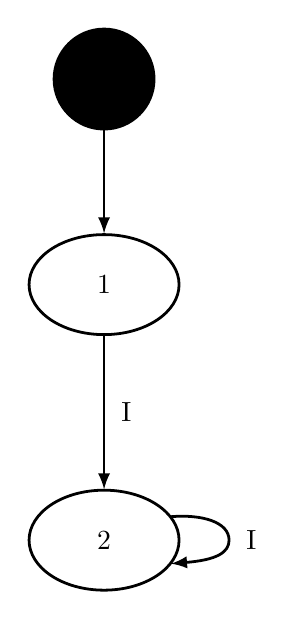
\begin{tikzpicture}[>=latex,line join=bevel,]
  \pgfsetlinewidth{1bp}
%%
\pgfsetcolor{black}
  % Edge: 0 -> 1
  \draw [->] (27.0bp,165.94bp) .. controls (27.0bp,157.81bp) and (27.0bp,147.88bp)  .. (27.0bp,128.44bp);
  % Edge: 1 -> 2
  \draw [->] (27.0bp,91.647bp) .. controls (27.0bp,78.823bp) and (27.0bp,61.108bp)  .. (27.0bp,36.3bp);
  \definecolor{strokecol}{rgb}{0.0,0.0,0.0};
  \pgfsetstrokecolor{strokecol}
  \draw (35.0bp,64.0bp) node {I};
  % Edge: 2 -> 2
  \draw [->] (51.074bp,26.454bp) .. controls (62.242bp,27.377bp) and (72.0bp,24.559bp)  .. (72.0bp,18.0bp) .. controls (72.0bp,13.593bp) and (67.595bp,10.875bp)  .. (51.074bp,9.5456bp);
  \draw (80.0bp,18.0bp) node {I};
  % Node: 1
\begin{scope}
  \definecolor{strokecol}{rgb}{0.0,0.0,0.0};
  \pgfsetstrokecolor{strokecol}
  \draw (27.0bp,110.0bp) ellipse (27.0bp and 18.0bp);
  \draw (27.0bp,110.0bp) node {1};
\end{scope}
  % Node: 0
\begin{scope}
  \definecolor{strokecol}{rgb}{0.0,0.0,0.0};
  \pgfsetstrokecolor{strokecol}
  \definecolor{fillcol}{rgb}{0.0,0.0,0.0};
  \pgfsetfillcolor{fillcol}
  \filldraw [opacity=1] (27.0bp,184.0bp) ellipse (18.0bp and 18.0bp);
\end{scope}
  % Node: 2
\begin{scope}
  \definecolor{strokecol}{rgb}{0.0,0.0,0.0};
  \pgfsetstrokecolor{strokecol}
  \draw (27.0bp,18.0bp) ellipse (27.0bp and 18.0bp);
  \draw (27.0bp,18.0bp) node {2};
\end{scope}
%
\end{tikzpicture}

